\SourcePage{229}{232}
\section{Calculation of semiclassical matrix elements}

Direct calculation of matrix elements of a physical quantity $f$ using
semiclassical wave functions presents serious difficulties. We assume that
the energies of the states connected by the matrix element are not close, so
the latter does not reduce to a Fourier component of $f$ (\secref{48}). The
difficulty arises because the exponential wave functions, with large
imaginary exponents, make the integrand rapidly oscillating.
\SourcePage{230}{233}
Consider one-dimensional motion in $U(x)$ and, for simplicity, let the
operator of $f$ be just a function of $x$. Let $\psi_1,\psi_2$ be real wave
functions for energies $E_1,E_2$, with $E_2>E_1$ (Fig.~17). We must calculate
\begin{equation}
 f_{12}=\int_{-\infty}^{+\infty}\psi_1f\psi_2\,dx. \tag{51.1}
\end{equation}

\begin{figure}[ht]
\centering
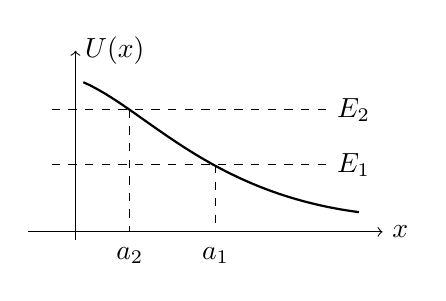
\begin{tikzpicture}[x=1cm,y=1cm]
 \draw[->] (-2.1,0)--(2.4,0) node[right] {$x$};
 \draw[->] (-1.5,-.1)--(-1.5,2.3) node[right] {$U(x)$};
 \draw[thick] (-1.4,1.9) .. controls (-.6,1.55) and (.2,.5) .. (2.1,.25);
 \draw[dashed] (-1.8,1.55)--(1.7,1.55) node[right] {$E_2$};
 \draw[dashed] (-1.8,.85)--(1.7,.85) node[right] {$E_1$};
 \draw[dashed] (-.81,1.55)--(-.81,0) node[below=2pt] {$a_2$};
 \draw[dashed] (.28,.85)--(.28,0) node[below=2pt] {$a_1$};
\end{tikzpicture}
\par\smallskip Fig. 17
\end{figure}

By (47.5), on the two sides of $x=a_1$ and sufficiently far from it,
\begin{equation}
 \psi_1=\begin{cases}
 \displaystyle\frac{C_1}{\sqrt{|p_1|}}
 \exp\left(-\frac1\hbar\int_x^{a_1}|p_1|\,dx\right),&x<a_1,\\[6pt]
 \displaystyle\frac{2C_1}{\sqrt{p_1}}
 \cos\left(\frac1\hbar\int_{a_1}^x p_1\,dx-\frac\pi4\right),&x>a_1,
 \end{cases} \tag{51.2}
\end{equation}
and similarly for $\psi_2$, with 1 replaced by 2.

Substitution of these asymptotic expressions in (51.1) would give a wrong
result. As shown below, the integral is exponentially small although its
integrand is not. A relatively small change in the integrand may therefore
change the order of the integral. This difficulty can be avoided as follows.

Write $\psi_2=\psi_2^++\psi_2^-$ by resolving the cosine for $x>a_2$ into two
exponentials. According to (50.2),
\SourcePage{231}{234}
\begin{equation}
 \psi_2^+=\begin{cases}
 \displaystyle\frac{-iC_2}{2\sqrt{|p_2|}}
 \exp\left(\frac1\hbar\int_x^{a_2}|p_2|\,dx\right),&x<a_2,\\[6pt]
 \displaystyle\frac{C_2}{2\sqrt{p_2}}
 \exp\left(\frac{i}{\hbar}\int_{a_2}^x p_2\,dx-\frac{i\pi}{4}\right),&x>a_2,
 \end{cases} \tag{51.3}
\end{equation}
and $\psi_2^-=(\psi_2^+)^*$.

Accordingly, (51.1) is the sum of two complex-conjugate integrals,
$f_{12}=f_{12}^++f_{12}^-$. The integral
\[
 f_{12}^+=\int_{-\infty}^{+\infty}\psi_1f\psi_2^+\,dx
\]
converges: although $\psi_2^+$ grows exponentially for $x<a_2$, $\psi_1$
decreases still faster for $x<a_1$, since $|p_1|>|p_2|$ throughout $x<a_2$.

Regard $x$ as complex and displace the integration path into the upper
half-plane. A positive imaginary increment of $x$ produces a growing term in
$\psi_1$ for $x>a_1$, but $\psi_2^+$ decreases faster because $p_2>p_1$
there. The integrand therefore decreases.

The displaced path no longer crosses $a_1,a_2$, where the semiclassical
approximation fails. Along the entire path we may use their asymptotic
expressions in the upper half-plane:
\begin{align}
 \psi_1&=\frac{C_1}{2[2m(U-E_1)]^{1/4}}
 \exp\left(\frac1\hbar\int_{a_1}^x\sqrt{2m(U-E_1)}\,dx\right),\notag\\
 \psi_2^+&=\frac{-iC_2}{2[2m(U-E_2)]^{1/4}}
 \exp\left(-\frac1\hbar\int_{a_2}^x\sqrt{2m(U-E_2)}\,dx\right), \tag{51.4}
\end{align}
\SourcePage{232}{235}
where the roots are chosen positive on the real axis for $x<a_2$. Thus
\begin{equation}
 \begin{split}
 f_{12}^+={}&\frac{-iC_1C_2}{4\sqrt{2m}}\int
 \exp\left[\frac1\hbar\int_{a_1}^x\sqrt{2m(U-E_1)}\,dx\right.\\
 &\left.{}-\frac1\hbar\int_{a_2}^x\sqrt{2m(U-E_2)}\,dx\right]
 \frac{f(x)\,dx}{[(U-E_1)(U-E_2)]^{1/4}}.
 \end{split}\tag{51.5}
\end{equation}
We seek to move the contour so as to reduce the exponential factor. Its
exponent has an extremum only where $U(x)=\infty$; for $E_1\ne E_2$ its
derivative vanishes nowhere else. The only restriction on moving the contour
upward is therefore the need to pass around the singular points of $U(x)$,
which, by the general theory of linear differential equations, are also the
singular points of $\psi(x)$.

\begin{figure}[ht]
\centering
\begin{tikzpicture}[x=1cm,y=1cm]
 \draw[->] (-1.5,0)--(1.8,0) node[right] {$x$};
 \fill (0,1.18) circle (1.3pt);
 \node[below] at (0,.92) {$x_0$};
 \draw[thick,->] (-.2,2.2)--(-.2,1.5);
 \draw[thick] (-.2,1.5)--(-.2,1.18) arc[start angle=180,end angle=360,radius=.2];
 \draw[thick,->] (.2,1.18)--(.2,2.05);
\end{tikzpicture}
\par\smallskip Fig. 18
\end{figure}

The contour depends on the form of $U(x)$. If $U$ has only one singular point
$x_0$ in the upper half-plane, the path may be chosen as in Fig.~18. The
immediate neighborhood of the singularity gives the principal contribution,
so $f_{12}=2\mathop{\rm Re}f_{12}^+$ is mainly proportional to
\begin{equation}
 f_{12}\sim\exp\left\{-\frac1\hbar\mathop{\rm Im}\left[
 \int^{x_0}\sqrt{2m(E_2-U)}\,dx-
 \int^{x_0}\sqrt{2m(E_1-U)}\,dx\right]\right\}. \tag{51.6}
\end{equation}
(L.~D. Landau, 1932).\footnote{Replacing the wave functions by their
asymptotic expressions in deriving (51.5), (51.6) is legitimate because the
order of the integral over the Fig.~18 contour is fixed by the order of its
integrand; a relatively small change of the latter has no material effect.}
The lower limits may be any points in classically accessible regions and do
not affect the imaginary
\SourcePage{233}{236}
parts. If $U(x)$ has several upper-half-plane singularities, $x_0$ in (51.6)
is the one giving the exponent of smallest absolute magnitude.\footnote{We
assume that $f(x)$ itself has no singularities. Estimate (51.6) also assumes
a prefactor of normal order. It may be anomalously small because of the
particular problem. The simplest example is $f(x)=\operatorname{const}$: the
matrix element vanishes by orthogonality, which (51.6) does not reveal.}

When $E_1,E_2$ are close, (51.6) simplifies and the matrix element reduces,
by \secref{48}, to a time Fourier component of the classical $f[x(t)]$. Put
$E_{2,1}=E\pm\hbar\omega_{21}/2$ and expand in $\hbar\omega_{21}$:
\begin{equation}
 f_{12}\sim\exp\left(-\omega_{21}\mathop{\rm Im}
 \int^{x_0}\frac{dx}{v}\right)=\exp(-\omega_{21}\mathop{\rm Im}\tau). \tag{51.6a}
\end{equation}
Here
\[
 \tau=\int^{x_0}\frac{dx}{v},\qquad v(x)=\sqrt{2(E-U(x))/m},
\]
may be viewed as the \emph{complex time} needed to reach $x_0$ in the complex
$x$ plane, and $v(x)$ as the corresponding ``complex velocity.'' Formula
(51.6a) indeed approximates the Fourier component when
$\omega_{21}\mathop{\rm Im}\tau\gg1$.

For motion in a central field the calculation is similar, but $U(r)$ is now
the effective potential energy, the sum of potential and centrifugal terms,
and differs for different $l$. For later use denote the two effective
potentials generally by $U_1(r),U_2(r)$. The exponent in the integrand of
(51.5) then has extrema not only at infinities of $U_1$ or $U_2$, but also at
points satisfying
\begin{equation}
 U_1(r)+U_2(r)=E_1+E_2. \tag{51.7}
\end{equation}
\SourcePage{234}{237}
Thus in
\begin{equation}
 f_{12}\sim\exp\left\{-\frac1\hbar\mathop{\rm Im}\left[
 \int^{r_0}\sqrt{2m(E_2-U_2)}\,dr-
 \int^{r_0}\sqrt{2m(E_1-U_1)}\,dr\right]\right\} \tag{51.8}
\end{equation}
the competing $r_0$ include both singular points and the roots of (51.7).

The central-field case also differs because the radial integral runs from 0,
not $-\infty$, to $+\infty$:
\[
 f_{12}=\int_0^\infty\chi_1f\chi_2\,dr.
\]
If the integrand is even, the range may formally be extended to the whole
axis and nothing changes. This can occur when $U_1,U_2$ are even. Then
$\chi_1,\chi_2$ are even or odd (see \secref{21}),\footnote{For even $U(r)$, the
radial wave function $R(r)$ is even (odd) for even (odd) $l$, as follows from
$R\sim r^l$ at small $r$.} and if $f(r)$ too is even or odd, their product may
be even. If the integrand is not even, as necessarily happens if $U(r)$ is
not even, the contour cannot be moved away from its initial point $r=0$, and
$r_0=0$ must also be included among the competing values in (51.8).

\begin{center}\textbf{Problems}\end{center}

\ProblemHeading{1.} Calculate the semiclassical matrix elements, retaining
only the exponential factor, in the field $U=U_0e^{-\alpha x}$.

\SolutionHeading The only infinity of $U(x)$ is at $x\to-\infty$, so put
$x_0=-\infty$ in (51.6), extending the integrals to $+\infty$. Each separately
diverges at $-\infty$; first integrate from $-x$ to $+\infty$ and then let
$x\to\infty$. The result is
\[
 f_{12}\sim\exp\left[-\frac{\pi m}{\alpha\hbar}(v_2-v_1)\right],
\]
\SourcePage{235}{238}
where $v_1=\sqrt{2E_1/m}$ and $v_2=\sqrt{2E_2/m}$ are the asymptotic free
velocities as $x\to\infty$.

\ProblemHeading{2.} Do the same in the Coulomb field $U=\alpha/r$ for
transitions between states with $l=0$.

\SolutionHeading The only singular point of $U(r)$ is $r=0$. The corresponding
integral was evaluated in Problem 2 of \secref{50}. Formula (51.8) gives
\[
 f_{12}\sim\exp\left[\frac{\pi\alpha}{\hbar}
 \left(\frac1{v_2}-\frac1{v_1}\right)\right].
\]

\ProblemHeading{3.} Do the same for an anharmonic oscillator with
\[
 U(x)=\frac{m\omega^2}{2}x^2+\beta x^4
\]
under the condition
\begin{equation}
 \hbar\omega\ll E_1,E_2\ll\frac{m^2\omega^4}{\beta}. \tag{1}
\end{equation}

\SolutionHeading Extension of the argument to finite motion shows that (51.6)
still applies. Choose $x_0\to\pm\infty$; both points contribute at the same
order. Thus
\[
 f_{12}\sim\exp\left\{-\frac1\hbar\left[
 \int_{a_2}^{-\infty}\sqrt{2m(U-E_2)}\,dx-
 \int_{a_1}^{-\infty}\sqrt{2m(U-E_1)}\,dx\right]\right\}.
\]
Under condition (1), the main contribution comes from
\begin{equation}
 \sqrt{\frac{E_1}{m\omega^2}},\sqrt{\frac{E_2}{m\omega^2}}\ll|x|\ll
 \sqrt{\frac{m\omega^2}{\beta}}, \tag{2}
\end{equation}
where
\[
 \frac{m\omega^2}{2}x^2\gg E_1,E_2,\beta x^4.
\]
Expanding the exponent in $E_{1,2}/U$, canceling the zeroth-order terms, and
neglecting $\beta x^4$, we obtain
\[
 f_{12}\sim\exp\left(-\frac{E_2}{\hbar\omega}\int\frac{d|x|}{|x|}
 +\frac{E_1}{\hbar\omega}\int\frac{d|x|}{|x|}\right).
\]
Cut off the logarithmic integrals at the boundaries of (2): above at
$x\sim\sqrt{m\omega^2/\beta}$ and below at
$x\sim a_{2,1}\sim\sqrt{E_{2,1}/(m\omega^2)}$. Then
\[
 f_{12}\sim\exp\left(-\frac{E_2}{2\hbar\omega}\ln\frac{m^2\omega^4}{\beta E_2}
 +\frac{E_1}{2\hbar\omega}\ln\frac{m^2\omega^4}{\beta E_1}\right).
\]
Introducing the state numbers
\[
 n_1\approx E_1/\hbar\omega,\qquad n_2\approx E_2/\hbar\omega,
\]
write the result as
\[
 f_{12}\sim\frac{n_2^{n_2/2}}{n_1^{n_1/2}}
 \left(\frac{\beta\hbar}{m\omega^3}\right)^{(n_2-n_1)/2}.
\]
\SourcePage{236}{239}
Since large $x$ are essential to the solution, this result applies when
$f(x)$ does not grow too rapidly at infinity. If $f(x)$ is a polynomial, its
degree must be small compared with $n_2-n_1$.
